\documentclass[12pt,runningheads]{article}
\usepackage[utf8]{inputenc}
\usepackage{amsmath,amssymb,hyperref,array,xcolor,multicol,verbatim,mathpazo}
\usepackage[normalem]{ulem}
\usepackage[pdftex]{graphicx}
\begin{document}

%%%% In most cases you won't need to edit anything above this line %%%%

\title{Assignment 1: Comet Trajectory\\GPGN 409}
\author{Garrett Sickles}
\maketitle
\subsection*{Introduction}
You are making observations of a comet in space to figure out if it is on a collision course with the Earth. For this you need to estimate as accurately as possible the trajectory of the comet. Your observations consist of coordinates $x$ and $y$ of the comet relative to the Sun at angles $\alpha$ measured with respect to a fixed point centrally located inside
the orbit (this information is not normally available, but it might make the solution to this assignment easier). The measurements have errors which you don’t know, but you have a way to estimate the measurement uncertainties. The problem is 2D, i.e. the comet, the Earth and all other planets are in the same plane.

\subsubsection*{Summary of Assumptions and Definitions}
\begin{enumerate}
\item Let the origin of the $X$-$Y$ coordinate system also be the location of the Sun.
\item Let the center of the comet's trajectory, as in the center of a circle or ellipse, be defined by the point in the $X$-$Y$ plane ($x_{o}$, $y_{o}$)
\item Let the trajectory of the comet be defined as a two dimensional ellipse not centered at the origin of the form
\begin{align*}
\frac{(x\ -\ x_{o})^2}{a^2}\ +\ \frac{(y-y_{o})^2}{b^2}\  =\ 1
\end{align*}
where $a$ and $b$ are the major and minor radii in the direction of the $X$ and $Y$ axes and \{$x$, $y$\} is the locus of all points that satisfy the above equation.
\item Let the angle of a point on the ellipse $\theta$ be defined as the angle traveling counter clockwise from the positive $X$ axis.
\item Let the formula for an inverse model be defined by the formulation of the least squares inversion where
\begin{align*}
\textbf{m}\ =\ (\textbf{G}^{\intercal}\textbf{W}^{\intercal}\textbf{W}\ \textbf{G})^{-1}\ \textbf{G}^{\intercal}\textbf{W}^{\intercal}\textbf{W}\ \textbf{d} \\
\end{align*}
as formulated and defined in homework 1.
\end{enumerate}

\subsubsection*{Summary of Data}
The data used in this problem was presented in the assignment and contains four types of data points, orthogonal measurements in astronomical units (AU) denoted by $x_{i}$ and $y_{i}$ which represent an observed location of the asteroid with respect to the Sun (the origin), an angle from the positive X axis to the recorded $X$-$Y$ point denoted by $\theta$, and uncertainty measurements denoted by $s_{i}$ representing a radius of uncertainty around some observation point.
\pagebreak

\subsection*{Formulation of the Forward Problem}
Given the equation for an ellipse not centered at the origin
\begin{align*}
\frac{(x\ -\ x_{o})^2}{a^2}\ +\ \frac{(y-y_{o})^2}{b^2}\  =\ 1
\end{align*}
we want to derive a formula where $x$ and $y$ are parameters of an angle $\theta$. To do this, consider the parametric equations
\begin{align*}
x(\theta)\ &=\ x_{o}\ +\ a\cos(\theta) \\
y(\theta)\ &=\ y_{o}\ +\ b\sin(\theta)
\end{align*}
which define an ellipse in the $X$-$Y$ plane as function of the variable $\theta$. By substituting this set of equations into the general equation of an ellipse
\begin{align*}
\frac{(x(\theta)\ -\ x_{o})^2}{a^2}\ &+\ \frac{(y(\theta)-y_{o})^2}{b^2}\  &=\ 1\\
\frac{((x_{o}\ +\ a\cos(\theta))\ -\ x_{o})^2}{a^2}\ &+\ \frac{((y_{o}\ +\ b\sin(\theta))-y_{o})^2}{b^2}\  &=\ 1\\
\frac{(a\cos(\theta))^2}{a^2}\ &+\ \frac{(b\sin(\theta))^2}{b^2}\ &=\ 1\\
\cos^{2}(\theta)\ &+\ \sin^{2}(\theta)\ &=\ 1
\end{align*}
we find that equation of an ellipse is valid as long as $a$ and $b$ are nonzero.
\pagebreak

\subsection*{A Rotated the Ellipse}
A more general solution for the equation of an ellipse can be found by applying a rotation matrix to the locus of points that define a two dimensional ellipse not centered at the origin with the major and minor axes parallel to the $X$ and $Y$ axes, respectively. The first step in this derivation is defining the rotation matrix $\textbf{R}$ of angle $\phi$, and the rotated location of our $X$ and $Y$ coordinates, $x'(\theta)$ and $y'(\theta)$, such that
\begin{align*}
\textbf{R}\ =\
\begin{bmatrix}
\ \cos(\phi)\ &\ -\sin(\phi)\ \\ 
\ \sin(\phi)\ &\ \cos(\phi)\ \\ 
\end{bmatrix},\\ \\
\vec{r}\ =\ 
\begin{bmatrix}
\ x(\theta)\ \ \\
\ y(\theta)\ \ \\
\end{bmatrix}\ =\ 
\begin{bmatrix}
\ a\cos(\theta)\ \ \\
\ b\sin(\theta)\ \ \\
\end{bmatrix}\ +\ 
\begin{bmatrix}
\ x_{o}\ \ \\
\ y_{o}\ \ \\
\end{bmatrix},
\end{align*}
and
\begin{align*}
\textbf{R}\ \vec{r}\  =\ \vec{r'}\ =\  
\begin{bmatrix}
\ x'(\theta)\ \ \\
\ y'(\theta)\ \ \\
\end{bmatrix}
\end{align*}
Expanding the expression above for the locus of points defining an ellipse parameterized by $x(\theta)$ and $y(\theta)$ yields the following equation for $x'(\theta)$ and $y'(\theta)$.
\begin{align*}
\textbf{R}\ \vec{r}\ &=\ 
\begin{bmatrix}
\ x'(\theta)\ \ \\
\ y'(\theta)\ \ \\
\end{bmatrix}\ =\ 
\begin{bmatrix}
\ \cos(\phi)\ &\ -\sin(\phi)\ \\ 
\ \sin(\phi)\ &\ \cos(\phi)\ \\ 
\end{bmatrix}\ 
\bigg( \begin{bmatrix}
\ a\cos(\theta)\ \ \\
\ b\sin(\theta)\ \ \\
\end{bmatrix}\ +\ 
\begin{bmatrix}
\ x_{o}\ \ \\
\ y_{o}\ \ \\
\end{bmatrix} \bigg) \\
\textbf{R}\ \vec{r}\ &=\ 
\begin{bmatrix}
\ x'(\theta)\ \ \\
\ y'(\theta)\ \ \\
\end{bmatrix}\ =\ 
\begin{bmatrix}
\ a\cos(\theta)\cos(\phi)\ -\ b\sin(\theta)\sin(\phi)\ \ \\
\ a\cos(\theta)\sin(\phi)\ +\ b\sin(\theta)\cos(\phi)\ \ \\
\end{bmatrix}\ +\ 
\begin{bmatrix}
\ x_{o}\cos(\phi)\ -\ y_{o}\sin(\phi)\ \ \\
\ x_{o}\sin(\phi)\ +\ y_{o}\cos(\phi)\ \ \\
\end{bmatrix}
\end{align*}
Thus there are two parametric equations in terms of $x'_{o}$, $y'_{o}$, $a$, $b$, $\theta$, and $\phi$ for the $X$ and $Y$ components of an ellipse, not centered at the origin and rotated by an angle $\phi$ about the origin. Note the rotated values corresponding to $x_{o}$ and $y_{o}$ are represented by $x'_{o}$ and $y'_{o}$.
\begin{align*}
\ x'(\theta)\ &=\ x'_{o}\ +\ a\cos(\theta)\cos(\phi)\ -\ b\sin(\theta)\sin(\phi)\ \\
\ y'(\theta)\ &=\ y'_{o}\ +\ a\cos(\theta)\sin(\phi)\ +\ b\sin(\theta)\cos(\phi)\ \\
\end{align*}
\pagebreak

\subsection*{Formulation of the Inverse Problem}
Using our formulation of the forward problem and the data presented in the assignment an inverse problem can be formulated. In fact we can perform a least squares inversion by formulating two similar inverse problems differentiated by the $X$ and $Y$ directions. After solving the inverse problems separately, the two models can be brought together to completely define an ellipse corresponding to the trajectory of the asteroid. From the equation for a model as defined in the least squares inversion we can define the quantities \textbf{W}, $\textbf{d}_{x}$, $\textbf{d}_{y}$, $\textbf{m}_{x}$, $\textbf{m}_{y}$, and \textbf{G} where \\
\begin{align*}
\textbf{G} &= 
\begin{bmatrix}
1 & \cos(\theta_{1}) & -\sin(\theta_{1})\\ \\
1 & \cos(\theta_{2}) & -\sin(\theta_{2})\\ \\
... & ... & ... \\ \\
1 & \cos(\theta_{N}) & -\sin(\theta_{N})\\
\end{bmatrix},\ 
\textbf{W} =  
\begin{bmatrix}
\ (w_{1})^{n} & 0 & 0\ \ \\ \\
\ 0 & ... & 0\ \ \\ \\
\ 0 & 0 & (w_{N})^{n}\ \ 
\end{bmatrix},\\ \\
\textbf{d}_{x} &= 
\begin{bmatrix}
\ x_{1} \ \\ \\
\ x_{2} \ \\ \\
\ ... \ \\ \\
\ x_{N} \ \\
\end{bmatrix},\ 
\textbf{d}_{y}= 
\begin{bmatrix}
\ y_{1} \ \\ \\
\ y_{2} \ \\ \\
\ ... \ \\ \\
\ y_{N} \ \\
\end{bmatrix},\  
\textbf{m}_{x}= 
\begin{bmatrix}
\ x'_{o} \ \ \\ \\
\ a\cos(\phi) \ \ \\ \\
\ -b\sin(\phi) \ \ \\
\end{bmatrix},\ 
\textbf{m}_{y}= 
\begin{bmatrix}
\ y'_{o} \ \ \\ \\
\ a\sin(\phi) \ \ \\ \\
\ b\cos(\phi) \ \ \\
\end{bmatrix}
\end{align*}

and
\begin{align*}
\textbf{m}_{x}\ &=\ (\textbf{G}^{\intercal}\textbf{W}^{\intercal}\textbf{W}\ \textbf{G})^{-1}\ \textbf{G}^{\intercal}\textbf{W}^{\intercal}\textbf{W}\ \textbf{d}_{x}\\
\textbf{m}_{y}\ &=\ (\textbf{G}^{\intercal}\textbf{W}^{\intercal}\textbf{W}\ \textbf{G})^{-1}\ \textbf{G}^{\intercal}\textbf{W}^{\intercal}\textbf{W}\ \textbf{d}_{y} \\
\end{align*} \\

\pagebreak
Using these two models, $\textbf{m}_{x}$ and $\textbf{m}_{y}$, the constant quantities $a$, $b$, and $\phi$ can be found relatively easily from the known quantities $a\cos(\phi)$, $a\sin(\phi)$, $b\cos(\phi)$, and $-b\sin(\phi)$.
\begin{align*}
\phi\ &=\ \arctan \bigg(\frac{a\sin(\phi)}{a\cos(\phi)}\bigg) \\
a\ &=\ \frac{a\sin(\phi)}{\sin(\phi)} \\
b\ &=\ \frac{b\cos(\phi)}{\cos(\phi)}
\end{align*}

\pagebreak
\subsection*{Inverting the Data}
Based on the data, the formulation of the forward problem, and the formulation of the inverse problem a deterministic inversion can was performed. This inversion was implemented in MatLab based on the formulations performed in previous sections of this assignment. Performing this operation yielded the following plot containing the raw data, an equally weighted inversion, and one alternative weighting scheme. The following table contains the model parameters in terms of $x_{o}$, $y_{o}$, $a$, $b$, and $\phi$ where the $n$ value corresponds to the exponent in the $(w_{i})^{n}$ term from the weighting matrix.
\begin{figure}[!h]
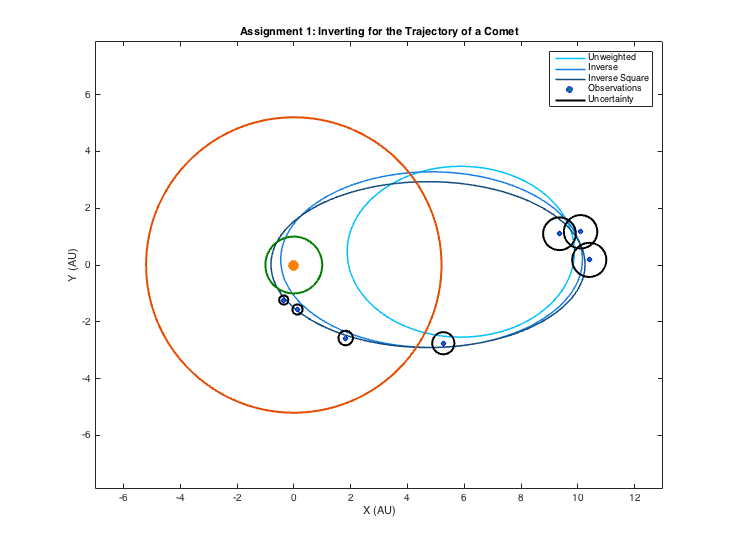
\includegraphics[width=\textwidth]{Trajectory.png}
\end{figure}
\begin{center}
\begin{tabular}{|c|rrrrrr|}
\hline
Color & $x_{0}$ (AU) & $y_{0}$ (AU) & $a$ (AU) & $b$ (AU) & $\phi(deg)$ & $n$ \\
\hline
\rule{0pt}{3ex} Light Blue (Unweighted)& $4.660$ & $-0.014$ & $5.633$ & $2.744$ & $1.339$ & $0$\\
Dark Blue ($\propto$ Area) & $4.697$ & $0.022$ & $5.541$ & $2.886$ & $0.422$ & $2.0$ \\
\hline
\end{tabular}
\end{center}

\pagebreak
\begin{figure}[!h]
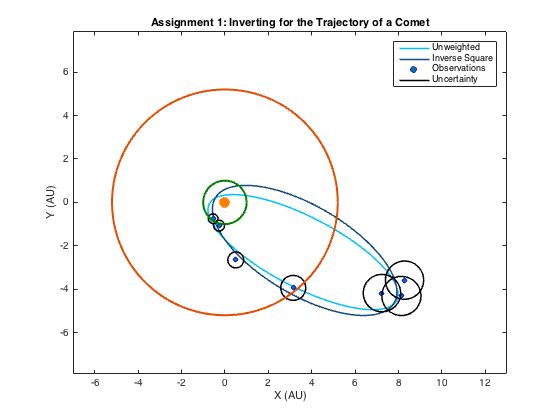
\includegraphics[width=\textwidth]{Trajectory1.png}
\end{figure}
\begin{center}
\begin{tabular}{|c|rrrrrr|}
\hline
Color & $x_{0}$ (AU) & $y_{0}$ (AU) & $a$ (AU) & $b$ (AU) & $\phi(deg)$ & $n$ \\
\hline
\rule{0pt}{3ex} Light Blue (Unweighted)& $3.597$ & $-2.293$ & $4.855$ & $1.607$ & $-27.402$ & $0$\\
Dark Blue ($\propto$ Area) & $3.676$ & $-2.214$ & $4.776$ & $2.027$ & $-30.672$ & $2.0$ \\
\hline
\end{tabular}
\end{center}

These plots show that weighting the data slightly can affect the trajectory of the comet. The inversion that equally weights the data points (light blue) could accurately reflect the shape each comet's trajectory but there are errors near the points of lowest uncertainty. The inversion which uses weights proportional to the area of uncertainty, that is the area inscribed by the circle of uncertainty surrounding each data point, appears to be the most accurate inversion because the trajectory intersects every area of uncertainty at each point. Both inversion techniques come close to the possible trajectories but the trajectory using weights proportional to the inverse of the square of uncertainty appear to be more realistic from the information provided.

\pagebreak
\section*{Appendix I: The Code}
\begin{verbatim}
function Comet_Trajectory(filename)
    [x, y, theta, s] = Import_Comet_Data(filename);
    G = [ones(length(s), 1) cosd(theta) sind(theta)];
    figure('Position', [100, 100, 700, 500]);
    Trajectory(LSWI(x,G,s,0), LSWI(y,G,s,0),strcat('0-',filename),...
        {'Color', [0 .76 1], 'LineWidth',1.5});
    Trajectory(LSWI(x,G,s,2.0),LSWI(y,G,s,2.0),strcat('2-',filename),...
        {'Color', [.08 .3 .5],'LineWidth',1.5});
    scatter(x,y,20,'MarkerEdgeColor','b',...
        'MarkerFaceColor',[0 .5 .5],'LineWidth',1.0); hold on;
    for i=1:length(s)
        Plot_Circle([x(i), y(i), s(i)],{'k','LineWidth',1.5});
    end
    plot(0, 0,'-ko','LineWidth',1,'MarkerEdgeColor',[1 .5 0],...
        'MarkerFaceColor',[1 .5 0],'MarkerSize',10); hold on;
    Plot_Circle([0, 0, 1],...
        {'Color', [0 0.5 0],'LineWidth',2});
    Plot_Circle([0, 0, 5.20],...
        {'Color', [.9 .3 0],'LineWidth',2})
    title(['Assignment 1: Inverting for the Trajectory of a Comet in ',...
        filename]);
    xlabel('X (AU)'); ylabel('Y (AU)');
    axis([-7,13,-7,7]); axis equal; 
    legend('Unweighted','Inverse Square','Observations','Uncertainty');
end
function [ x, y, theta, sigma ] = Import_Comet_Data(filename)
    data = importdata(filename);
    d = data.data;
    x = d(:,1);
    y = d(:,2);
    theta = d(:,3);
    sigma = d(:,4);
end
function [ m ] = LSWI(d, G, w, n)
    W = diag(1./(w.^(n)));
    m = pinv((G')*(W')*(W)*(G))*(G')*(W')*(W)*(d);
end
function [ h, k, a, b, p ] = Ellipse_Parameters(mx, my, filename)
    file = fopen(['Solved-', filename], 'w');
    h = mx(1); k = my(1);
    p = atan2d(my(2), mx(2));
    a = mx(2)./cosd(p); b = my(3)./cosd(p);
    fprintf(file, 'mx: %f, %f, %f\nmy: %f, %f, %f\n',...
        mx(1), mx(2), mx(3), my(1), my(2), my(3));
    fprintf(file,'h: %f\nk: %f\na: %f\nb: %f\nPhi: %f\n',...
        h, k, a, b, p);
    fclose(file);
end
function Trajectory(mx, my, id, param)
    t=0.0:0.001:2*3.1415926;
    Ellipse_Parameters(mx, my, id);
    plot(mx(1)+mx(2)*cos(t)+mx(3)*sin(t),...
        my(1)+my(2)*cos(t)+my(3)*sin(t),...
        param{:}); hold on;
end
function Plot_Circle(m, param)
    t=0.0:0.001:2*3.1415926;
    plot(m(1)+m(3).*cos(t),m(2)+m(3).*sin(t), param{:}); hold on;
end
\end{verbatim}

\end{document}